\subsection{Medidor de espesores por ultrasonido}
\label{sec:ut-calibracion}

\subsubsection{Instrumento, patrón y condiciones ambientales}

El medidor calibrado es el INSIZE ISU-100D, descrito en la
Sección~\ref{sec:instr-ut} \parencite{insize_isu100d}.

\vspace{6pt}
Procedimiento por comparación con instrumento de referencia según la norma PC-029
del INACAL \parencite{inacal_pc029} (\textit{Procedimiento para la calibración de
medidores de espesores por ultrasonido}), con la técnica de eco de pulso descrita
en la Sección~\ref{sec:ut}.

\vspace{12pt}
\subsubsection*{Equipos e instrumentos utilizados:}
\begin{tabular}{ll}
Patrón escalonado de acero & \\[3pt]
Glicerina (gel acoplante)  & \\[3pt]
Mesa de planitud           & \\[3pt]
Termómetro de contacto     & Exactitud $\pm 0.5\ ^\circ\text{C}$
\end{tabular}

\vspace{12pt}
\subsubsection*{Nomenclatura:}
\begin{tabular}{ll}
$VP$        & Valor patrón del escalón\\[3pt]
$\bar e_k$  & Indicación media del medidor en el punto $k$\\[3pt]
$E_k$       & Error de indicación en el punto $k$\\[3pt]
$V_{PE}$    & Valor certificado del patrón de espesor\\[3pt]
$\alpha$    & Coeficiente de dilatación del acero\\[3pt]
$\Delta T_i$ & Desviación térmica de la pieza respecto de $20\ ^\circ\text{C}$\\[3pt]
$\delta l_{res}$ & Corrección por resolución del display
\end{tabular}

\subsubsection{Datos experimentales}
\label{sec:ut-datos}

Se ensayan diez espesores del patrón escalonado, de $2.50$ a $25.00$ mm en pasos de
$2.50$ mm, con cinco lecturas repetidas por punto. El error de indicación elemental
se calcula como

\begin{equation}
    E_k = \left(\bar e_k - VP_k\right)\times 1000\ \mu\text{m},
    \label{eq:ut-E-simple}
\end{equation}

donde $\bar e_k$ es la media de las cinco lecturas. La temperatura del ensayo varió
de $22.5$ a $23.3\ ^\circ\text{C}$. La Tabla~\ref{tab:ut-datos} recoge las
mediciones y la Tabla~\ref{tab:ut-estadistica} su reducción estadística elemental.

\begin{table}[H]
\centering
\caption{Mediciones de calibración del medidor de espesores por ultrasonido: cinco lecturas repetidas por valor patrón del escalón.}
\label{tab:ut-datos}
\begin{tabular}{rrrrrrr}
\toprule
$N$ & $VP$ (mm) & $e_1$ (mm) & $e_2$ (mm) & $e_3$ (mm) & $e_4$ (mm) & $e_5$ (mm) \\
\midrule
1 & 2.50 & 2.51 & 2.50 & 2.51 & 2.51 & 2.50 \\
2 & 5.00 & 5.05 & 4.98 & 5.00 & 4.98 & 4.98 \\
3 & 7.50 & 7.47 & 7.54 & 7.53 & 7.51 & 7.49 \\
4 & 10.00 & 10.00 & 9.98 & 10.01 & 10.01 & 10.01 \\
5 & 12.50 & 12.54 & 12.52 & 12.51 & 12.51 & 12.50 \\
6 & 15.00 & 15.01 & 15.00 & 14.99 & 14.96 & 14.99 \\
7 & 17.50 & 17.52 & 17.55 & 17.47 & 17.46 & 17.49 \\
8 & 20.00 & 20.01 & 19.99 & 19.98 & 19.97 & 20.02 \\
9 & 22.50 & 22.52 & 22.54 & 22.52 & 22.48 & 22.53 \\
10 & 25.00 & 25.05 & 25.03 & 25.00 & 24.99 & 24.97 \\
\bottomrule
\end{tabular}
\end{table}


\begin{table}[H]
\centering
\caption{Cálculo estadístico elemental por punto de calibración. $\bar e$ es la media de las cinco lecturas, $s$ la desviación estándar muestral y $E$ el error de indicación sin correcciones.}
\label{tab:ut-estadistica}
\begin{tabular}{rrrrr}
\toprule
$VP$ (mm) & $\bar e$ (mm) & $s$ ($\mu$m) & $s/\sqrt{n}$ ($\mu$m) & $E$ ($\mu$m) \\
\midrule
2.50 & 2.506 & 5.48 & 2.45 & 6 \\
5.00 & 4.998 & 30.33 & 13.56 & -2 \\
7.50 & 7.508 & 28.64 & 12.81 & 8 \\
10.00 & 10.002 & 13.04 & 5.83 & 2 \\
12.50 & 12.516 & 15.17 & 6.78 & 16 \\
15.00 & 14.990 & 18.71 & 8.37 & -10 \\
17.50 & 17.498 & 37.01 & 16.55 & -2 \\
20.00 & 19.994 & 20.74 & 9.27 & -6 \\
22.50 & 22.518 & 22.80 & 10.20 & 18 \\
25.00 & 25.008 & 31.94 & 14.28 & 8 \\
\bottomrule
\end{tabular}
\end{table}


El error de indicación máximo es $E_{\max} = 18\ \mu\text{m}$, en $22.50$ mm, y el
mínimo $E_{\min} = -10\ \mu\text{m}$, en $15.00$ mm, de modo que el alcance del
error en el intervalo ensayado es

\begin{equation}
    f_e = E_{\max} - E_{\min} = 18 - (-10) = 28\ \mu\text{m}.
    \label{eq:ut-fe}
\end{equation}

\subsubsection{Deducción de las ecuaciones de medición e incertidumbre}

El espesor indicado se obtiene del tiempo de vuelo de la onda,
$e = c_L \Delta t / 2$, ecuación~\eqref{eq:espesor-tof}. Al compararlo con el valor
del patrón y corregir la dilatación lineal de ambos cuerpos respecto de
$T_0 = 20\ ^\circ\text{C}$,

\begin{equation}
  E = \bar e\left(1 - \alpha_{inst} \Delta T_{inst}\right)
    - V_{PE}\left(1 - \alpha_{PE} \Delta T_{PE}\right).
  \label{eq:ut-e-termal}
\end{equation}

Con $\bar e \approx V_{PE}$ en los términos correctivos y un único coeficiente
$\alpha$ para el acero, la expresión linealizada es

\begin{equation}
  E = f(\bar e;\, \delta l_{res};\, V_{PE};\, \alpha;\, \Delta T_i)
  = \bar e - V_{PE} - V_{PE}\,\alpha\,\Delta T_i ,
  \label{eq:ut-e-model}
\end{equation}

donde $\delta l_{res}$ entra como corrección aditiva de la indicación. La función
depende de cinco variables independientes, por lo que su varianza se obtiene con la
ley de propagación de la ecuación~\eqref{eq:error-std-values}. Evaluando los
coeficientes de sensibilidad $c_j = \partial E / \partial x_j$ en el vector de
valores medios,

\begin{align}
  c_1 &= \ptij{E}{\bar e} = 1, &
  c_2 &= \ptij{E}{\delta l_{res}} = 1, \nonumber \\
  c_3 &= \ptij{E}{V_{PE}} = -\left(1 + \alpha\,\Delta T_i\right), \label{eq:ut-sens} \\
  c_4 &= \ptij{E}{\alpha} = -V_{PE}\,\Delta T_i, &
  c_5 &= \ptij{E}{\Delta T_i} = -V_{PE}\,\alpha . \nonumber
\end{align}

Sustituyendo~\eqref{eq:ut-sens} en la ley de propagación, con
$\text{Cov}(x_i, x_j) = 0$ para $i \neq j$, la varianza combinada del error de
indicación resulta

\begin{align}
  u_c^2(E) &=
  u^2(\bar e) + u^2(\delta l_{res})
  + \left[1 + \alpha\,\Delta T_i\right]^2 u^2(V_{PE}) \nonumber \\
  &\quad + \left[V_{PE}\,\Delta T_i\right]^2 u^2(\alpha)
  + \left[V_{PE}\,\alpha\right]^2 u^2(\Delta T_i).
  \label{eq:ut-sigma}
\end{align}

\subsubsection{Componentes de incertidumbre del error de indicación}

La repetibilidad es la única evaluación tipo~A y se obtiene de las cinco lecturas
repetidas de cada punto, conforme a la
ecuación~\eqref{eq:sigma-media-experimental}:

\begin{equation}
  u(\bar e_k) = \frac{s_k}{\sqrt{5}},
  \qquad
  s_k^2 = \frac{1}{4} \sum_{p=1}^{5} \left(e_{kp} - \bar e_k\right)^2 .
  \label{eq:ut-sigma-LL}
\end{equation}

El máximo se alcanza en $17.50$ mm, donde
$u(\bar e) = 16.55\ \mu\text{m}$; el mínimo, en $2.50$ mm, con
$u(\bar e) = 2.45\ \mu\text{m}$ (Tabla~\ref{tab:ut-estadistica}).

Las componentes restantes son evaluaciones tipo~B. La resolución de la pantalla,
$r = 0.01$ mm, se acota con la distribución rectangular de la
ecuación~\eqref{eq:sigma-rectangular}:

\begin{equation}
  u(\delta l_{res}) = \frac{r}{2\sqrt{3}} = \frac{0.01}{\sqrt{12}}\ \text{mm}
  \approx 2.89\ \mu\text{m}.
  \label{eq:ut-sigma-res}
\end{equation}

La incertidumbre del patrón escalonado combina el certificado de calibración, con
$U_{cert} = 0.05$ mm y $k = 2$, y la deriva dimensional máxima
$U_{der} = 0.1$ mm tratada como rectangular:

\begin{equation}
  u^2(V_{PE}) = \left(\frac{U_{cert}}{k}\right)^2
  + \frac{U_{der}^2}{3},
  \label{eq:ut-sigma-PE}
\end{equation}

de donde

\begin{equation}
  u(V_{PE}) = \sqrt{\left(\frac{0.05}{2}\right)^2 + \frac{0.1^2}{3}}\ \text{mm}
  \approx 62.9\ \mu\text{m}.
  \label{eq:ut-sigma-PE-valor}
\end{equation}

Esta componente es casi siete veces mayor que la repetibilidad del instrumento y
domina el balance final. Para el coeficiente de dilatación del acero,
$\alpha = 11.5\times10^{-6}\ ^\circ\text{C}^{-1}$ con una tolerancia del $10\ \%$,

\begin{equation}
  u(\alpha) = \frac{0.1\,\alpha}{\sqrt{3}}
  \approx 6.7\times10^{-7}\ ^\circ\text{C}^{-1}.
  \label{eq:ut-sigma-alpha}
\end{equation}

Finalmente, con la exactitud del termómetro $U_{Tcert} = 0.5\ ^\circ\text{C}$
($k = 2$) y la fluctuación observada $\Delta t_A = 0.8\ ^\circ\text{C}$,

\begin{equation}
  u(\Delta T_i) = \sqrt{\left(\frac{U_{Tcert}}{k}\right)^2
  + \left(\frac{\Delta t_A}{\sqrt{3}}\right)^2}\ ^\circ\text{C}
  \approx 0.53\ ^\circ\text{C}.
  \label{eq:ut-sigma-dT}
\end{equation}

Con $\Delta T_i = 2.9\ ^\circ\text{C}$ en el centro del intervalo térmico, el
coeficiente que multiplica a $u(V_{PE})$ vale
$c_3 = 1 + \alpha\Delta T_i = 1.000033$.

\subsubsection{Simplificación y resultado final}
\label{sec:ut-simplificacion}

Los dos términos térmicos de~\eqref{eq:ut-sigma} son los únicos que dependen del
espesor. En el extremo del alcance valen

\begin{align}
  \left[V_{PE}\,\Delta T_i\right]^2 u^2(\alpha)
  &\approx 1.1\times10^{-3}\ \mu\text{m}^2, \label{eq:ut-term-alpha} \\
  \left[V_{PE}\,\alpha\right]^2 u^2(\Delta T_i)
  &\approx 1.1\times10^{-2}\ \mu\text{m}^2, \label{eq:ut-term-dT}
\end{align}

es decir, menos del $0.001\ \%$ de la varianza combinada. Por lo tanto,

\begin{equation}
  u_c^2(E) \approx u^2(\bar e) + u^2(\delta l_{res})
  + c_3^2\,u^2(V_{PE}),
  \qquad
  U(E) = 2\,u_c(E),
  \label{eq:ut-U}
\end{equation}

con factor de cobertura $k = 2$ \parencite{jcgm2008gum, inacal_pc029}.

Como referencia, tomando la repetibilidad del punto más desfavorable
($u(\bar e) = 16.55\ \mu\text{m}$) para todo el alcance, la forma cerrada
queda

\begin{equation}
  U(E,L) = \sqrt{1.70\times10^{4} + 1.61\times10^{-4}\,L^2}\ \mu\text{m},
  \label{eq:ut-U-vecL}
\end{equation}

con $L$ en milímetros. El término cuadrático aporta apenas
$0.10\ \mu\text{m}^2$ en $L = 25$ mm, de modo que $U(E)$ es prácticamente
constante con el espesor: la variación que se observa punto a punto proviene de la
repetibilidad y no de la longitud.

\subsubsection{Resultados numéricos de la calibración}
\label{sec:ut-resultados}

\begin{table}[H]
\centering
\caption{Componentes de incertidumbre típica y resultados de la calibración punto a punto. Los términos térmicos se detallan en la Tabla~\ref{tab:ut-balance}.}
\label{tab:ut-componentes}
\begin{tabular}{rrrrrr}
\toprule
$VP$ (mm) & $u(\bar e)$ ($\mu$m) & $c_3\,u(V_{PE})$ ($\mu$m) & $u(\delta l_{res})$ ($\mu$m) & $u_c(E)$ ($\mu$m) & $U(E)$ ($\mu$m) \\
\midrule
2.50 & 2.45 & 62.92 & 2.89 & 63.03 & 126.1 \\
5.00 & 13.56 & 62.92 & 2.89 & 64.43 & 128.9 \\
7.50 & 12.81 & 62.92 & 2.89 & 64.27 & 128.5 \\
10.00 & 5.83 & 62.92 & 2.89 & 63.25 & 126.5 \\
12.50 & 6.78 & 62.92 & 2.89 & 63.35 & 126.7 \\
15.00 & 8.37 & 62.92 & 2.89 & 63.54 & 127.1 \\
17.50 & 16.55 & 62.92 & 2.89 & 65.12 & 130.2 \\
20.00 & 9.27 & 62.92 & 2.89 & 63.66 & 127.3 \\
22.50 & 10.20 & 62.92 & 2.89 & 63.80 & 127.6 \\
25.00 & 14.28 & 62.92 & 2.89 & 64.58 & 129.2 \\
\bottomrule
\end{tabular}
\end{table}


La incertidumbre expandida crece de $126.1\ \mu\text{m}$, en $2.50$ mm, a
$130.2\ \mu\text{m}$, en $17.50$ mm. El balance del punto más desfavorable se
muestra en la Tabla~\ref{tab:ut-balance}: el $93.3\ \%$ de la varianza proviene de
la deriva del patrón escalonado, seguida de la repetibilidad ($6.5\ \%$) y de la
resolución ($0.2\ \%$); los términos térmicos no alcanzan el $0.001\ \%$.

\begin{table}[H]
\centering
\caption{Balance de incertidumbre del error de indicación en el punto de mayor repetibilidad (17.50 mm).}
\label{tab:ut-balance}
\begin{tabular}{lrrr}
\toprule
Contribución & $u_i$ ($\mu$m) & $u_i^2$ ($\mu$m$^2$) & Peso en la varianza (\%) \\
\midrule
$u(\bar e)$ (repetibilidad) & 16.553 & 274.0000 & 6.46 \\
$u(\delta l_{res})$ (resolución) & 2.887 & 8.3333 & 0.20 \\
$c_3\,u(V_{PE})$ (patrón) & 62.917 & 3958.5974 & 93.34 \\
$(V_{PE}\Delta T_i)\,u(\alpha)$ & 0.034 & 0.0011 & $<0.01$ \\
$(V_{PE}\alpha)\,u(\Delta T_i)$ & 0.106 & 0.0112 & $<0.01$ \\
$u_c(E)$ & 65.12 & 4240.94 & 100.00 \\
$U(E) = 2\,u_c(E)$ & 130.25 & — & — \\
\bottomrule
\end{tabular}
\end{table}


\begin{figure}[H]
\centering
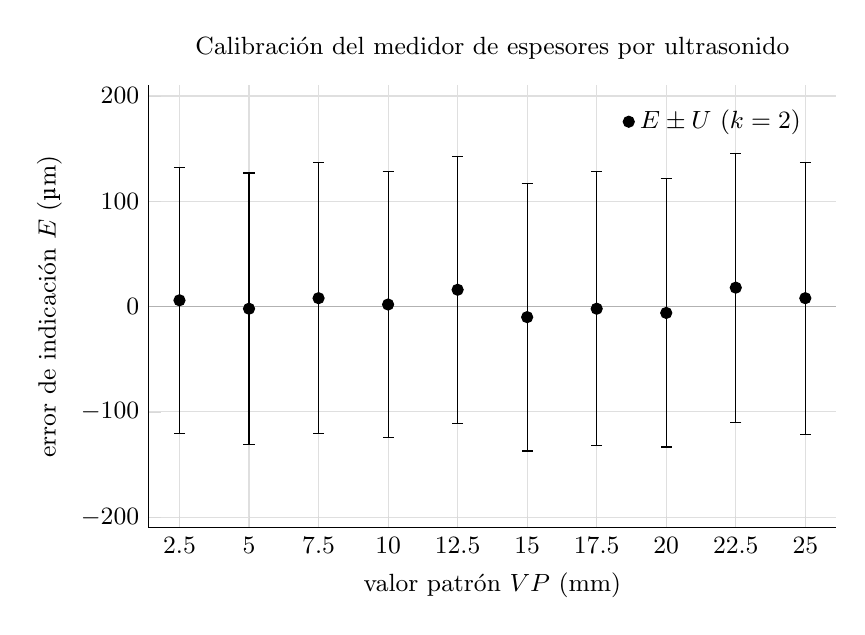
\begin{tikzpicture}
\begin{axis}[
  width=.85\textwidth,
  height=7.2cm,
  title={Calibración del medidor de espesores por ultrasonido},
  xlabel={valor patrón $VP$ (mm)},
  ylabel={error de indicación $E$ (µm)},
  xmin=1.4, xmax=26.1,
  ymin=-210, ymax=210,
  xtick={2.5,5,7.5,10,12.5,15,17.5,20,22.5,25},
  xticklabel style={/pgf/number format/.cd,fixed,precision=1},
  ytick={-200,-100,0,100,200},
  axis lines*=left,
  grid=major,
  grid style={gray!25},
  tick style={gray!30},
  legend pos=north east,
  legend style={draw=none, fill=none, font=\small},
  legend cell align={left},
  font=\small,
]
\draw[gray!60] (axis cs:1.4,0) -- (axis cs:26.1,0);
\addplot[
  only marks,
  mark=*,
  mark options={black},
  error bars/y dir=both,
  error bars/y explicit,
] table[x=VP, y=E, y error=U] {
  VP    E     U
  2.5   6     126.1
  5.0   -2    128.9
  7.5   8     128.5
  10.0  2     126.5
  12.5  16    126.7
  15.0  -10   127.1
  17.5  -2    130.2
  20.0  -6    127.3
  22.5  18    127.6
  25.0  8     129.2
};
\addlegendentry{$E \pm U$ ($k=2$)}
\end{axis}
\end{tikzpicture}
\caption{Error de indicación del medidor de espesores por ultrasonido e
incertidumbre expandida ($k=2$) en cada valor patrón.}
\label{fig:ut-error-U}
\end{figure}

El reparto de la Tabla~\ref{tab:ut-balance} explica el resultado: la incertidumbre
está gobernada por el patrón y no por el instrumento. Con un patrón de menor deriva,
la incertidumbre del ISU-100D descendería hasta el orden de su repetibilidad, del
orden de $10\ \mu\text{m}$. Los términos térmicos, en cambio, no alteran el balance
porque la pieza y el patrón son del mismo acero y están a la misma temperatura,
igual que se verificó en la calibración del pie de rey.
